\documentclass{article}
\usepackage{graphicx}
\usepackage{amsmath}

\begin{document}

\begin{equation*}
\Omega _i =[-w_x, w_x] \times [-w_y, w_y] \times [0,H]
\end{equation*}
\begin{equation*}
\Omega _o=[-W_x, W_x] \times [-W_y, W_y] \times [0,H]
\end{equation*}

\begin{equation*}
u_i=\left( \frac{z}{H} \right)^2 sin(\frac{\pi}{H}z) sin(\frac{\pi}{w_x}x) sin(\frac{\pi}{w_y}y)
\end{equation*}

\begin{equation*}
u_o= u_i + cos (\pi (x-w_x)(x+w_x)) cos(\pi (y- w_y)(y+w_y))
\end{equation*}
\begin{figure}
\center
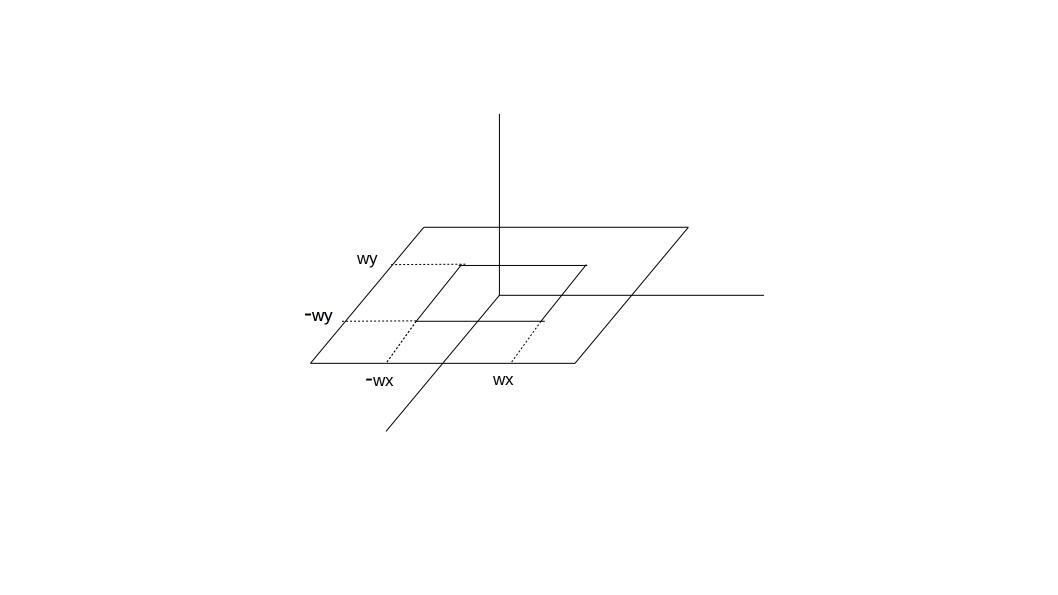
\includegraphics[scale=0.5]{bm.jpg}
\end{figure}
The solution satisfies the following:

\begin{eqnarray*}
u_o -u_i \neq 0\\
{\nabla u_i \cdot n_i }_{|\Gamma} + {\nabla u_o \cdot n_o} _{|\Gamma} =0\\
{\nabla u_i \cdot n_i} _{|\Gamma} \neq 0 
\end{eqnarray*}
\end{document}